\begin{frame}
\frametitle{Likelihood and Uncertainty Quantification}

\small

The posterior probability is obtained by maximizing the multivariate Gaussian likelihood.

\vspace{0.2cm}

\[
\mathcal{L}(\theta)
\propto
\exp\!\left[
-\frac12
(\mathbf y_m-\mathbf y_e)^T
\Sigma^{-1}
(\mathbf y_m-\mathbf y_e)
\right]
\]

\vspace{-0.1cm}

\[
\Sigma=\Sigma_{\rm exp}+\Sigma_{\rm emu}+\Sigma_{\rm model}
\]

\vspace{0.3cm}

\begin{columns}[T]

\column{0.48\textwidth}

\textbf{Experimental covariance}

\[
\Sigma_{\rm exp}
=
\Sigma_{\rm stat}
+
\Sigma_{\rm sys}
\]

\begin{itemize}
\item Statistical uncertainty
\item Correlated systematic uncertainty
\end{itemize}

\column{0.48\textwidth}

\textbf{Model covariance}

\[
\Sigma_{\rm model}
=
\Sigma_{\rm pred}
+
\Sigma_{\rm stat}^{\rm model}
+
\Sigma_{\rm sys}^{\rm model}
\]

\begin{itemize}
\item Emulator prediction
\item Simulation statistics
\item Model discrepancy
\end{itemize}

\end{columns}

\vfill

{\tiny
Adapted from Bernhard \emph{et al.},
Nature Physics 15 (2019).
}

\end{frame}


\begin{frame}
\frametitle{Effect of the Experimental Covariance}

\begin{columns}[T]

%%%%%%%%%%%%%%%%%%%%%%%%%%%%%%%%%%%%

\column{0.42\textwidth}

\small

Our study focuses on the experimental systematic covariance,

\[
\boxed{\Sigma_{\rm sys}}
\]

which determines how systematic uncertainties are correlated among experimental data points.

\vspace{0.3cm}

Different covariance models are investigated:

\begin{itemize}
\item Diagonal
\item Compound Symmetry
\item Radial Basis Function (RBF)
\end{itemize}

\vspace{0.3cm}

Changing $\Sigma_{\rm sys}$ modifies the likelihood and therefore the posterior constraints.

%%%%%%%%%%%%%%%%%%%%%%%%%%%%%%%%%%%%

\column{0.58\textwidth}

\centering

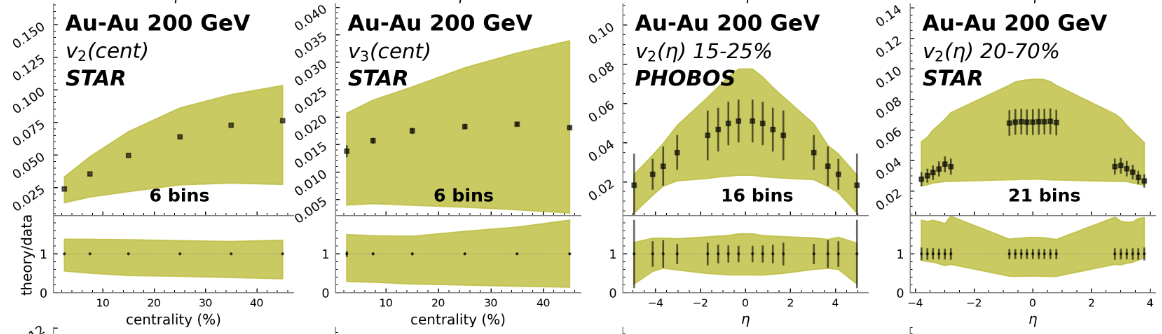
\includegraphics[width=.95\linewidth]{img/Au-Au-prior.png}

\vspace{0.15cm}

{\Large $\Downarrow$}

\small Bayesian calibration

\vspace{0.15cm}

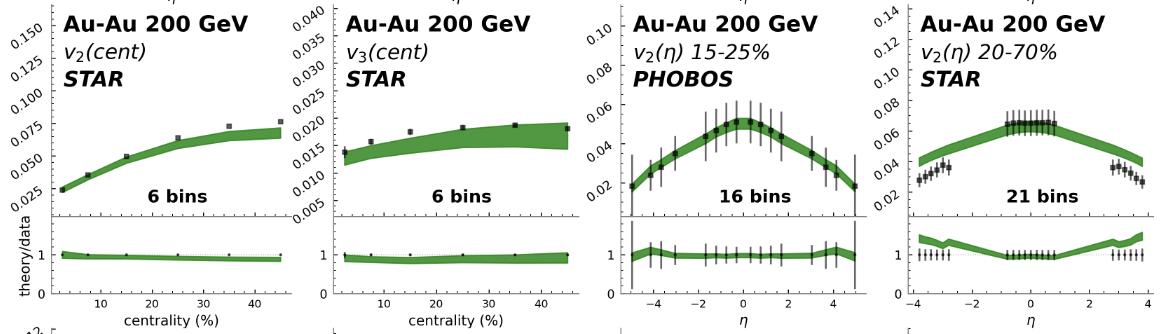
\includegraphics[width=.95\linewidth]{img/Au-Au-posterior.png}

\end{columns}

\end{frame}